\begin{frame}{Marco teórico}{\textcolor{UniBlue}{.}}
\begin{itemize}
	\item Ejemplo de Cadena de Markov
\end{itemize}

\begin{figure}[p]
	\centering
	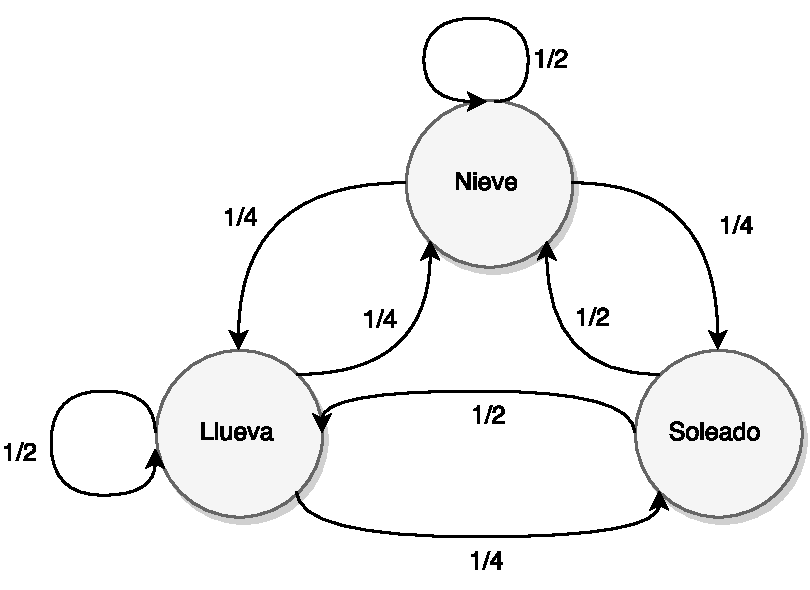
\includegraphics[scale=0.5]{images/EjCadenaMarkov.pdf}
\end{figure}

\end{frame}

\begin{frame}{Marco teórico}{\textcolor{UniBlue}{.}}
\begin{itemize}
	\item Ejemplo de Cadena de Markov reductible
\end{itemize}

\begin{figure}[p]
	\centering
	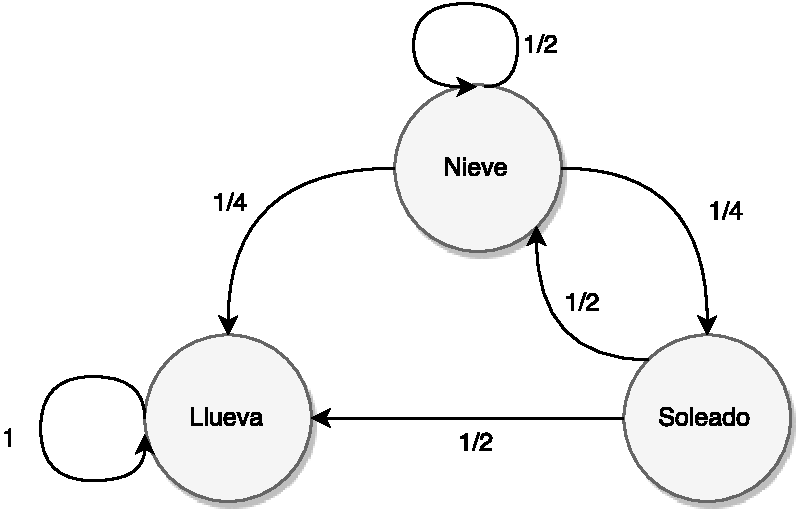
\includegraphics[scale=0.5]{images/EjCadenaMarkov-Reductible.pdf}
\end{figure}

\end{frame}

\begin{frame}{Marco teórico}{\textcolor{UniBlue}{.}}
\begin{itemize}
	\item Ejemplo de Cadena de Markov aperíodica
\end{itemize}

\begin{figure}[p]
	\centering
	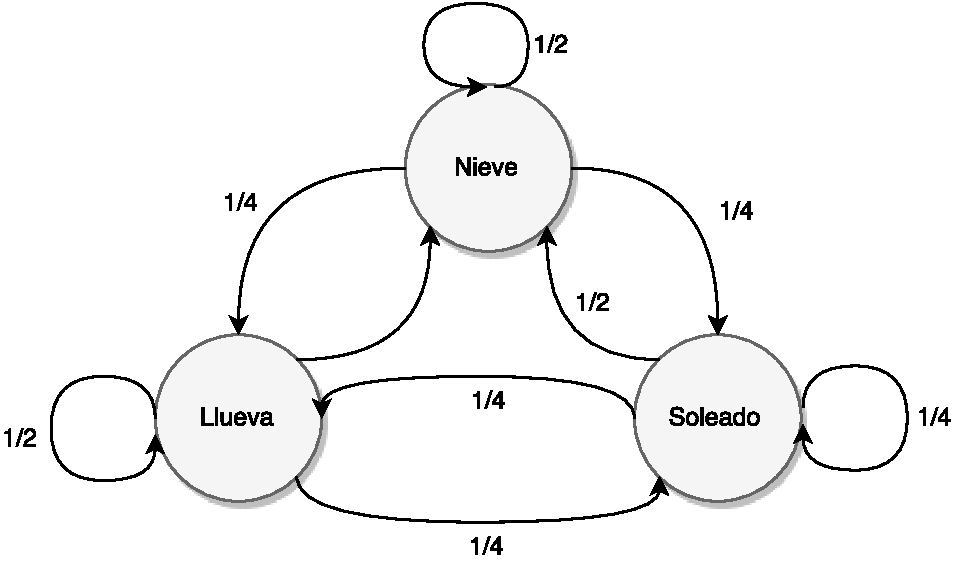
\includegraphics[scale=0.5]{images/EjCadenaMarkov-Aperiodica.pdf}
\end{figure}

\end{frame}